\documentclass{report}
\usepackage{graphicx}
\usepackage{todonotes}
\usepackage{hyperref}

\def\thesection{\arabic{section}}

\begin{document}

\title{Plant Simulation Lab Report}
\author{
	Auer, Philipp-Alexander\\
	\texttt{e1420446@student.tuwien.ac.at}
	\and
	Breitenfellner, Claudia\\
	\texttt{e8526042@student.tuwien.ac.at}
}

\maketitle
\tableofcontents
\pagebreak
\section{Introduction}
In this Lab Report we will present the results of our simulation based on the production facility used in the Information Technology in Automation lecture. The model consists of 6 Stations as described by the course material. The model was implemented in PlantSimulation\footnote{\url{https://www.plant-simulation.de/}} and after an initial version was completed we conducted several experiments to give some insight on how the factory will behave in different (hypothetical) scenarios.
Our model just assumes a Drill and DrillCheck Module, which should on this abstract level not make any difference. 
Furthermore: In the real-world model all of the EndStorage Modules have actual capacities and need to be emptied manually. While this makes sense in the context of the real-world factory, we want to simulate over longer times and test the throughput limits of the model, so we just model them as infinitely large sinks.
\section{Implementation Overview}
The first task was to implement a model, which assumes optimal parameters. Those parameters where determined using plain experimentation s.t. bottlenecks do not occur. For a visual representation of the PlantSimulation model see figure \ref{fig:overview}.
\begin{figure}[h!]
	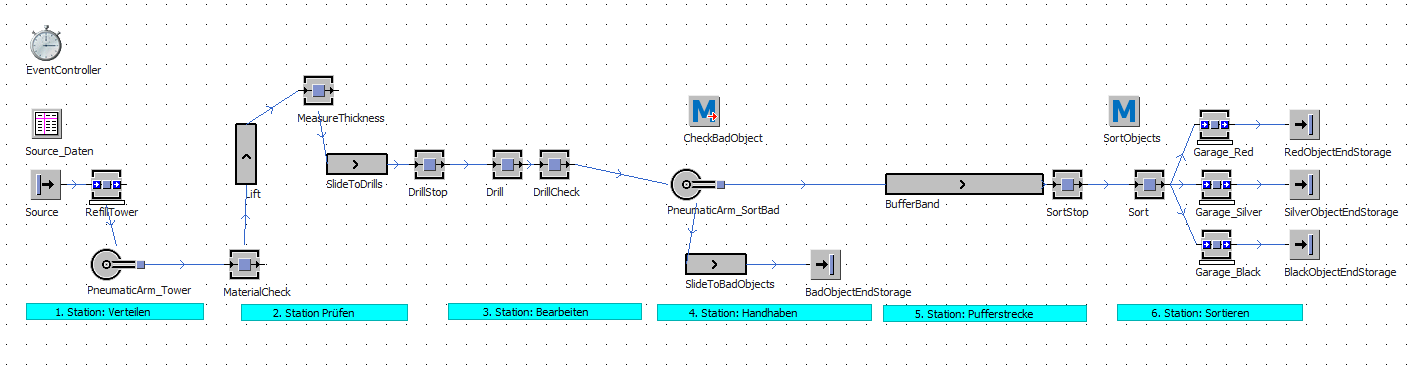
\includegraphics[width=\textwidth]{figures/overview.png}
	\caption{Top-Level overview of the PlantSimulation Model}
	\label{fig:overview}
\end{figure}
A few Notes on the details of this simulation: The drilling module in the real-world is some sort of turntable, which PlantSimulation knows as well, but our slot has 4 slots, while we could not model that in PlantSimulation. Station 2 is able to detect parts that are too thick, and has a way to get rid of them via a slide. While this behavior is implied with the "MeasureThickness" we think that the particular behavior of the real-world factory (where thick parts need to be moved down again via the lift) is a huge potential bottleneck.
\section{Results}
In the following section you can find some experimental results we found when simulating different scenarios. The scenarios and outcomes are described briefly, at the end of the document you can find a detailed Resource Statistics Report. 
\subsection{Assuming optimal parameters}
The first scenario assumes that we have complete control over the parameters of the simulated factory. 
While this is not the case it gives us some good baseline data. As can be seen in Figure \ref{fig:stat-optimal}, 
there are no bottlenecks in this scneario, though even if it was possible to design our real-world factory like that, 
we can observe in the statistics, that most of the machinery would have to idle a big percentage of the time.

\subsection{Assuming realistic parameters}
This scenario assumes an already existing real-world implementation in form of the video included in the course material.
While this is not typically possible in the planning phase of a project, it gives some insight on what can really cause 
bottlenecks in a real-world implementation. It is getting a lot more interesting than the plain optimal model. 
We can observe that \texttt{MaterialCheck} blocks a lot of the time, though this might as well be a result of the model not being fully accurate, 
\texttt{MaterialCheck} and \texttt{PneumaticArm\_Tower} being a bit too fast. We can also see, that station 3 consisting of the \texttt{Drill} 
is most likely going to be a bottleneck, while the end of the assembly line gets a lot of idle time.

\subsection{Assuming small buffer}
The purpose of station 5 is to act as a buffer. 
This scenario assumes that this buffer is very small and can only take one piece at a time, 
otherwise it assumes the same parameters as the optimal scenario. The results can be seen in Figure \ref{fig:stat-optimal-low-buf} and
show the immense effect the Buffer has on the whole factory. By limiting the amount of elements it can carry to 1, 
the whole drill operation starts to bottleneck.

\subsection{Assuming more performant drill station}
With additional financial power we can enhance the production process and make drilling twice as fast, 
eighter by using better material and machinery, or by parallelizing the process.
This model uses realistic parameters, but the Drill and DrillCheck modules operate twice as fast. What we observed here was, 
improving the performance of the drill station, we cannot fully resolve all bottlenecks and the increase in throughput per hour is only marginal.
For a more detailled report view the auxillary PlantSimulation model in\\\texttt{Projekt\_Sortieranlage\_2D\_realistic\_fast\_drill.spp} you should have received with this document.
\section{Attachments}
\begin{figure}[h!]
	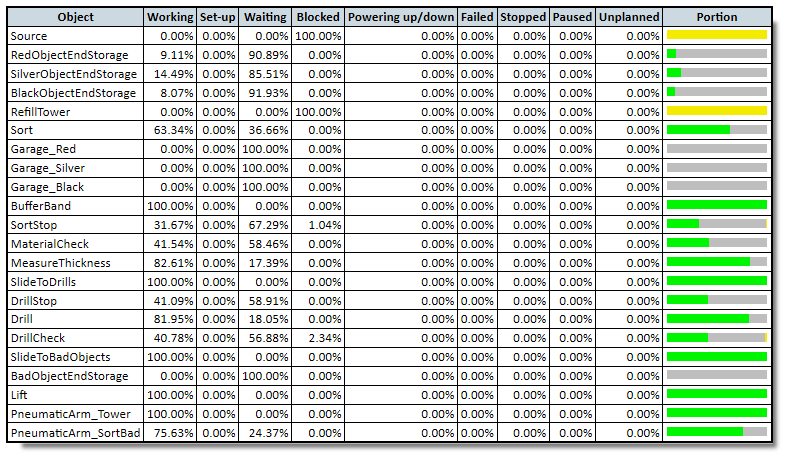
\includegraphics[width=\textwidth]{figures/stat-optimal.png}
	\caption{Optimal parameters without bottlenecks}
	\label{fig:stat-optimal}
\end{figure}
\begin{figure}[h!]
	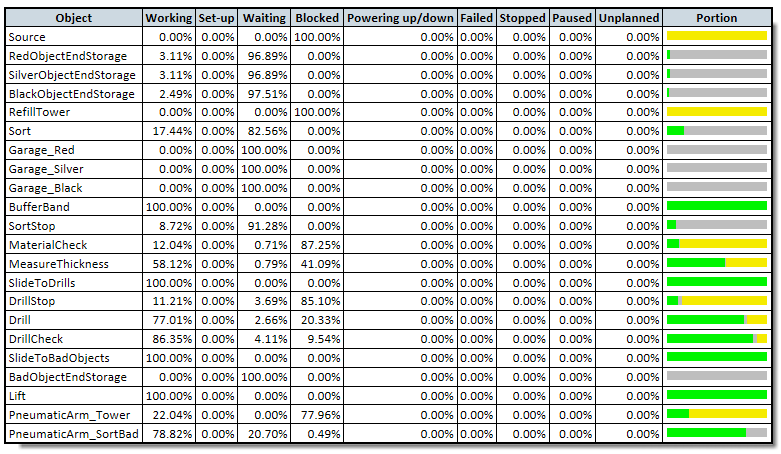
\includegraphics[width=\textwidth]{figures/stat-realistic.png}
	\caption{Realistic parameters according to video in the course material}
	\label{fig:stat-realistic}
\end{figure}
\begin{figure}[h!]
	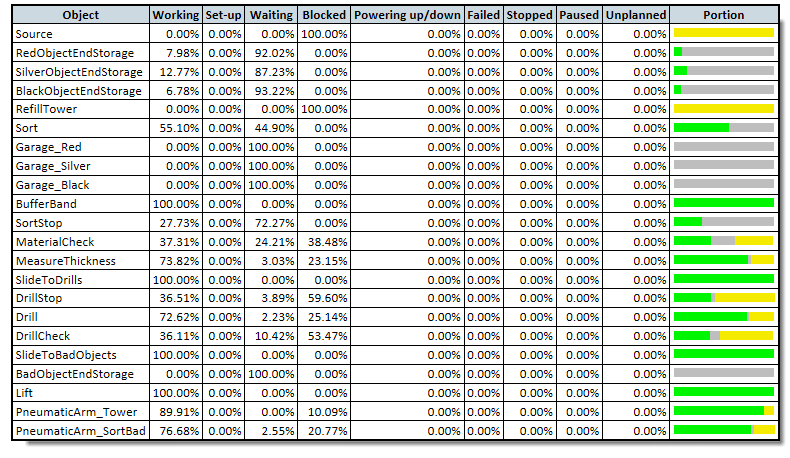
\includegraphics[width=\textwidth]{figures/stat-optimal-low-buf.png}
	\caption{Optimal parameters, BufferBand can only carry one element}
	\label{fig:stat-optimal-low-buf}
\end{figure}
\end{document}